\chapter{Specialized Cloud Mechanisms}
Abbiamo visto i meccanismi di base, ora passiamo ai meccanismi specializzati, che si appoggiano su quelli visti prima. Rappresentano uno stato superiore ai meccanismi di cui sopra e possono essere combinati in maniera diversa come parte di un'architettura specializzata per fornire un certo tipo di servizio. Nella figura 

\section{Automated Scaling Listener}
È un service agent che monitora e traccia le comunicazioni tra i consumer e i servizi cloud per uno scaling dinamico delle risorse. I listeneres sono all'interno del Cloud e tengono traccia automaticamente delle informazioni sul carico di lavoro, il quale viene determinato in modo grezzo (ad esempio byte/secondo) o dalla semantica delle richieste. Ci sono due diversi tipi di risposta al variare del carico di lavoro:
\begin{itemize}
    \item \textbf{Auto-scaling}: scala automaticamente le risorse IT basandosi sui parametri precedentemente definiti dal cloud consumer. Visto che il carico può aumentare in maniera significativa, occorre prendere in considerazione il fatto che i prezzi potrebbero aumentare inaspettatamente.
    \item \textbf{Notification}: inviare una notifica  quando i carichi di lavoro eccedono i limiti impostati oppure scendono al di sotto delle risorse allocate. 
\end{itemize}
In figura è mostrato un esempio: supponiamo di avere abbastanza risorse per 3 utenti (consumer) che dopo aver passato un firewall incontrano la componente di automated scaling listener che si occupa di servire le istanze del servizio allocate sulla macchina virtuale e contemporaneamente di monitorare quello che succede. Quando entra in gioco un quarto customer, lo scaling listener avvisa il CLoud resource administrator che è in grado di allocare maggiori risorse per soddisfare tutti gli utenti.



\subsubsection{\textbf{Caso d'uso: DTGOV}}
I server fisici scalano verticalmente dalla configurazione più bassa (1 vCPU, 4GB RAM) a quella più alta (128 vCPU 512GB RAM) automaticamente. Viene fatto scale up ogni volta che la VIM alloca 3 server virtuali e aumenta l'utilizzo della CPU all'80\% per 60 secondi. Se non è possibile scalare virtualmente, viene migrata la macchina virtuale su un'altra macchina fisica meno carica per alleggerire il carico di lavoro e tenere le prestazioni alte. Lo scale down avviene quando la VIM diminuisce le prestazioni di RAM e CPU al 15\% per 60 secondi. Il service agent che si occupa di rilevare questi cambi è appunto l'Automatic Scaling listener.

\section{Load Balancer}
Se l'ASL si occupa di scalare verticalmente, il Load Balancer è un meccanismo che si occupa dello scaling orizzontale: bilancia infatti i carichi di lavoro tra differenti risorse. Un Load Balancer può utilizzare diverse strategie in base al carico di lavoro:
\begin{itemize}
    \item \textbf{Asymmetric Distribution} - utilizzata in caso di risorse eterogenee, assegna i carichi di lavoro più onerosi alle risorse con più capacità di calcolo.
    \item \textbf{Workload Prioritization} - assegna i carichi di lavoro in base alle priorità delle richieste.
    \item \textbf{Content-Aware Distribution} - il carico di lavoro viene assegnato in base al contenuto della richiesta.
\end{itemize}
I Load Balancer usano un insieme di parametri di performance e qualità del servizio per ottimizzare l'utilizzo delle risorse IT, ed il loro scopo è massimizzare le richieste e minimizzare l'uso delle risorse.

Di solito il Load Balancer si trova tra consumer e provider, ovvero tra chi genera il carico di lavoro e tra chi lo processa. Può essere trasparente, come dei proxy al livello 7 della pila ISO/OSI. Scambia richieste esattamente come dovrebbero essere scambiate. Può essere anche un dispositivo hardware, come uno switch multilayer.

\section{SLA Monitor}
È un meccanismo che ha particolare interesse nell'ambito del management: osserva le performance di un servizio per stabilire se sono rispettati i requisiti di QoS stabiliti nel Service Level Agreement. I dati raccolti dal SLA monitor sono processati da un \textit{SLA Management System} per essere aggregate nelle statistiche di un SLA. Risulta anche utile a segnalare servizi o risorse in stato \textit{down}\footnote{Per servizio down non si intende solo un server che non risponde o una risorsa non disponibile. Anche aspettare 12 secondi per caricare una pagina HTML può essere considerato una condizione di down, perché è un tempo troppo lungo in normali condizioni.}, per permettere al sistema di ripararle o sostituirle.

Si comporta come un agente di polling, che invia dei messaggi di richiesta e memorizza le risposte in un database di log. Se i messaggi riportano un problema, il SLA monitor riporta una condizione di down.

\subsubsection{\textbf{Caso d'uso: DTGOV}}
La minima percentuale di availability per DTGOV è del 99.95\%. È tracciata usando due SLA monitor: uno basato su un polling agent e l'altro su un normale monitoring agent. Mentre il polling agent controlla con timeout di 20 secondi che tutti i servizi siano disponibili, il monitoring agent viene implementato direttamente dalla VIM, quindi agisce a stretto contatto con le risorse. Gli eventi generati dal polling agent hanno una marca temporale e sono salvati in un DB di log e poi utilizzati dal SLA Management System per calcolare l'availability delle risorse.

\section{Pay-per-use Monitor}
È collegato al precedente, perché raccoglie anch'esso informazioni, non per controllare la qualità del servizio offerto ma per calcolare il prezzo da pagare per la qualità offerta. Tipicamente controlla la quantità di richieste e di risposte, il volume dei dati trasferiti ed il consumo di banda (quindi relativo al tempo). I dati raccolti dal Pay-per-use monitor sono processati da un Billing Management System che calcola le quote da pagare.

\subsubsection{\textbf{Caso d'uso: DTGOV}}
DTGOV ha un sistema commerciale che può generare fatture basate sugli eventi. Ha due database proprietari, uno dove salva gli eventi di billing e uno dove salva lo schema dei prezzi. Gli eventi a runtime sono raccolti tramite cloud usage monitor che sono implementati come estensioni della piattaforma VIM utilizzando le sue API.

\section{Audit Monitor}
L'audit monitor si occupa di verificare la correttezza dei dati e delle procedure: il suo utilizzo è reso necessario da obblighi contrattuali e regolatori. È implementato come un monitoring agent che intercetta le richieste di accesso e salva le credenziali di sicurezza del richiedente, i tentativi di accesso riusciti o falliti, in un database, per eventuali utilizzi futuri.


\section{Failover System}
È un meccanismo utilizzato per aumentare la reliability e l'availability delle risorse utilizzando tecnologie di clustering per fornire implementazioni ridondanti. È configurato per switchare su una risorsa copiata o in standby nel caso di malfunzionamento di un'altra risorsa ed è spesso utilizzato nel caso di presenza di \textit{single point of failure}. Ci sono due tipi di configurazioni:
\begin{itemize}
    \item \textbf{Active/Active} - le risorse ridondanti vengono fornite e servite contemporaneamente, ne viene utilizzata una sola solo in caso di fallimento dell'altra.
    \item \textbf{Active/Passive} - viene utilizzata una risorsa, mentre l'altra viene utilizzata solo in caso di malfunzionamento della prima, spostando il carico di lavoro su di essa.
\end{itemize}

\section{Hypervisor}
Come abbiamo già visto, l'Hypervisor è una parte fondamentale per la virtualizzazione di di un'infrastruttura, per generare risorse virtuali anzichè risorse fisiche. Il suo utilizzo è limitato ad una singola macchina, e ha capacità funzionali limitate. Il software di un hypervisor può essere installato su qualsiasi macchina

\section{Resource Cluster}
Le risorse IT cloud-based possono essere combinate logicamente per migliorare la loro allocazione e il loro utilizzo. Il meccanismo di \textbf{Resource Cluster} viene usato per raggruppare diverse istanze di risorse IT in modo che possano operare come una singola risorsa: questo aumenta la capacità computazionale, il bilanciamento del carico, e l'availability delle risorse stesse. Ci sono diversi meccanismi di \textit{clusterizzazione}:
\begin{itemize}
    \item \textbf{Server Cluster} - server fisici o virtuali sono raggruppati in cluster per aumentare le performance e l'availability. Gli hypervisor girano su diversi server fisici e possono essere configurati per condividere gli stati di esecuzione al fine di creare dei server virtuali clusterizzati.
    \item \textbf{Database Cluster} - pensati per migliorare l'availability dei dati: hanno una feature di sincronizzazione che permette la consistenza dei dati, i quali sono conservati fisicamente in dispositivi diversi.
    \item \textbf{Large Dataset Cluster} - i dati vengono partizionati e distribuiti in modo da aumentare l'efficienza senza compromettere la precisione e di calcolo o l'integrità degli stessi.
\end{itemize}
Inoltre, ci sono due tipi di resource cluster:
\begin{itemize}
    \item \textbf{Load Balancer Cluster} - specializzato in carichi di lavoro molto pesanti, aumentano la capacità delle risorse preservando la gestione centralizzata delle risorse IT grazie a un load balancer.
    \item \textbf{High Availability Cluster} - mantiene la disponibilità del sistema anche a seguito di fallimento di nodi, grazie al resource replication.
\end{itemize}
\section{Multi-device Broker}
Un cloud service potrebbe essere utilizzato da un insieme di cloud consumer che sono differenziati dai loro dispositivi di hosting e/o requisiti di comunicazione. Per risolvere problemi di compatibilità tra un cloud service e diversi cloud service consumer, bisogna convertire le informazioni che si scambiano a runtime. Il meccanismo di \textit{multi-device broker} è utilizzato per facilitare questa trasformazione in modo che i servizi siano accessibili ad un range più ampio di cloud consumer.

\begin{figure}[ht]
    \centering
    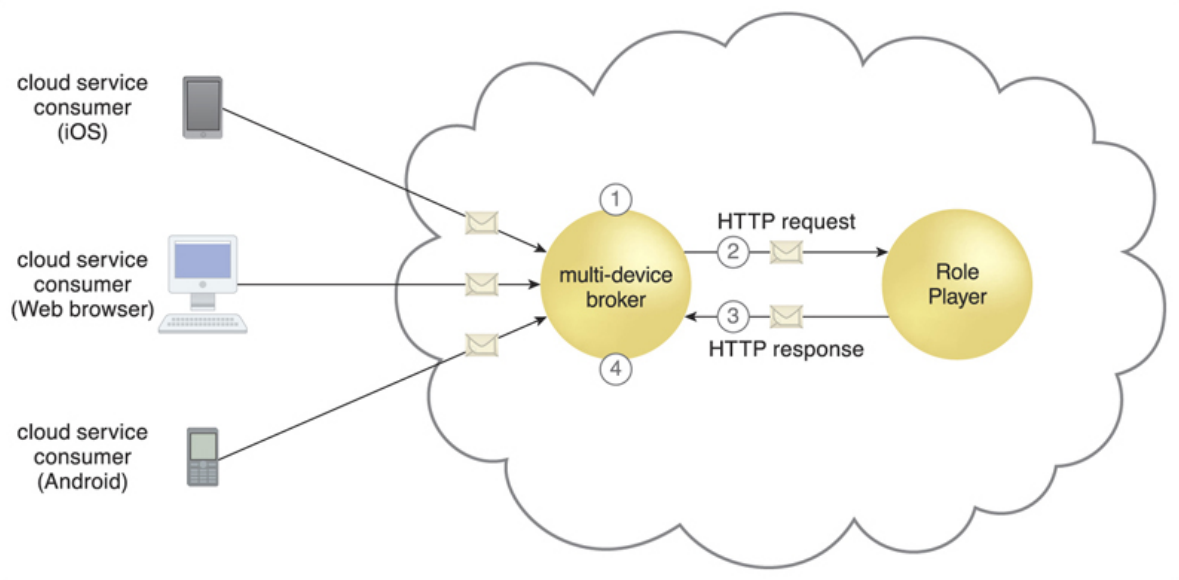
\includegraphics[width=10cm]{./Images/cap9/9.3.png}
\end{figure}

\section{State Management Database}
È un dispositivo di storage utilizzato per conservare temporaneamente i dati persistenti dei software che vengono utilizzati. Può essere visto come un'alternativa al meccanismo di caching, e in più la scalabilità del sistema è aumentata: infatti non sempre i dati di un servizio devono essere utilizzati al 100\%, ed è per questo che questo meccanismo risulta importante.

\begin{figure}[ht]
    \centering
    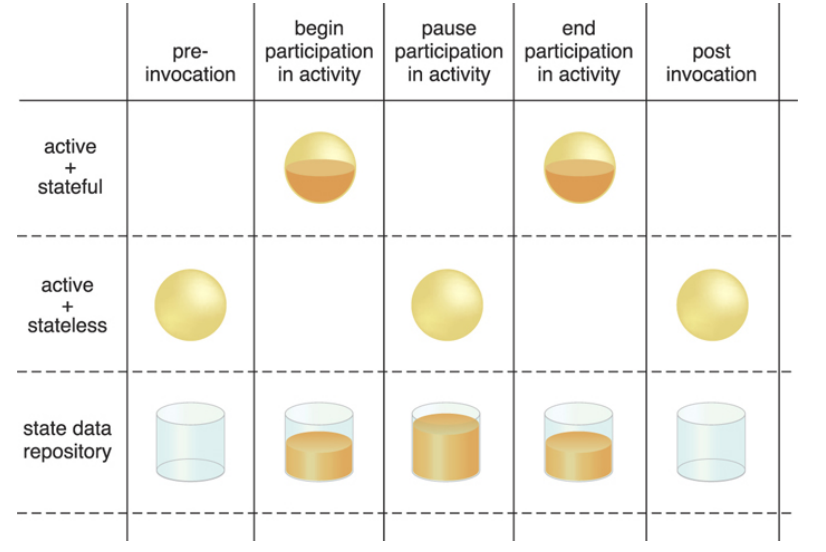
\includegraphics[width=9cm]{./Images/cap9/9.4.png}
\end{figure}



\section{Mappa concettuale delle caratteristiche del Cloud Computing}

\begin{figure}[ht]
    \centering
    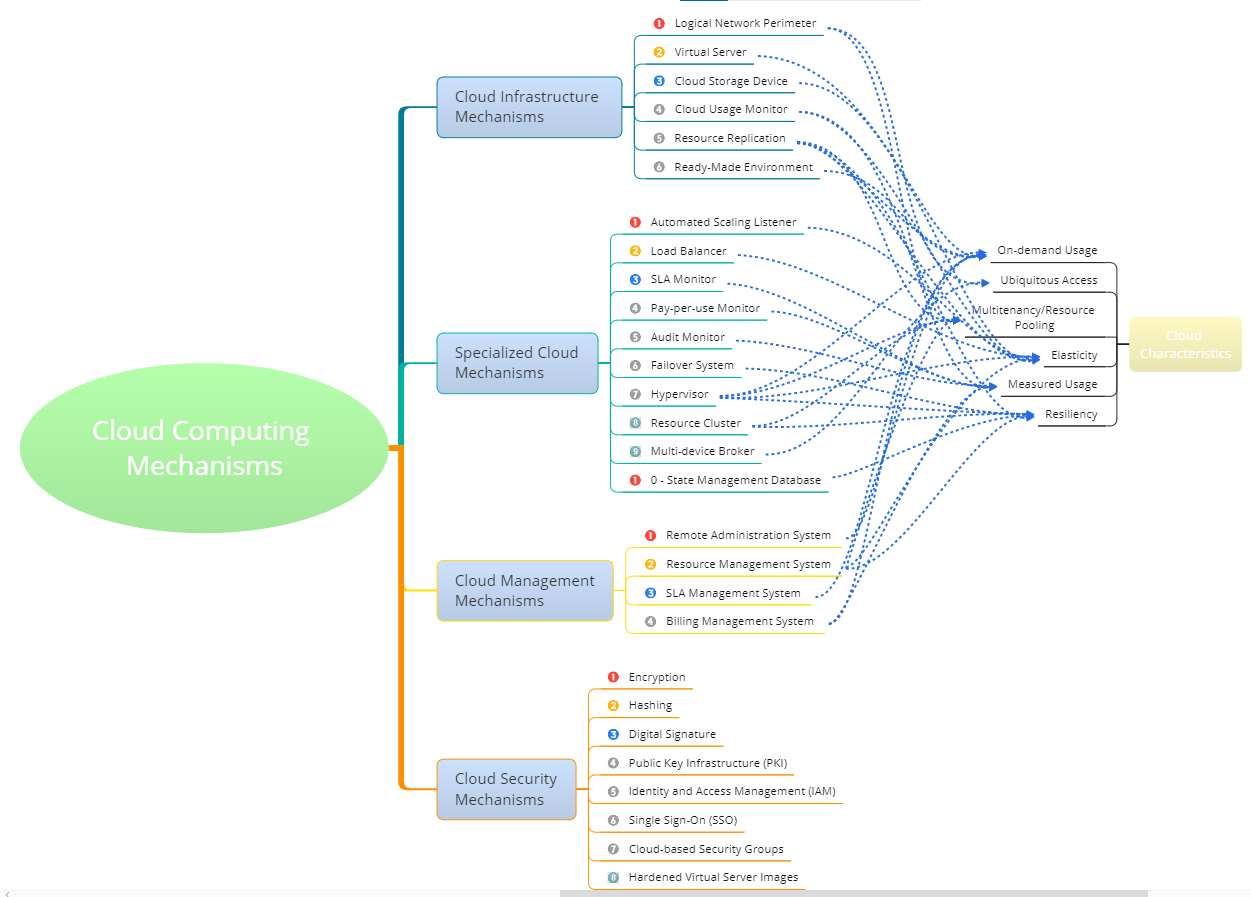
\includegraphics[width=12cm]{./Images/cap9/9.1.png}
\end{figure}

\section{Learning Check}
\begin{enumerate}
    \item Descrivi il meccanismo dell'Automated Scaling Listener e spiega le due risposte comuni che questo meccanismo può avere in base alle condizioni di carico.
    \item Descrivi gli obiettivi del meccanismo del Load Balancer, elenca le tre funzioni base di bilanciamento del carico e spiega in che modo un load balancer viene posizionato all'interno dell'architettura cloud.
    \item Descrivi gli obiettivi del meccanismo di SLA Monitor e spiega l'importanza del monitoring dell'utilizzo in relazione con un SLA e alle garanzie pubblicate in esso.
    \item Descrivi il meccanismo e spiega come è in relazione con la fatturazione del cloud provider.
    \item Descrivi gli obiettivi del meccanismo Audit Monitor e spiega la sua importanza nelle regolamentazioni di carattere legale.
    \item Descrivi il funzionamento del meccanismo di Failover System e spiega la sua relazione con le tecnologie di clustering.
    \item Descrivi gli obiettivi del meccanismo di Hypervisor e spiega la sua relazione con il meccanismo di virtual server. Inoltre spiega che relazione c'è tra l'Hypervisor e un virtual server.
    \item Descrivi gli obiettivi del meccanismo di Resource CLuster e spiega come funzionano le risorse raggruppate in cluster. Inoltre spiega la differenza tra cluster che possiedono high availability da quelli sottoposti a bilanciamento del carico.
    \item Descrivi il meccanismo di Multi-Device Broker e spiega come utilizza le tecnologie del cloud per supportare l'accesso a diversi cloud service da parte dei cloud consumer.
    \item Descrivi il meccanismo di State Management Database e la sua importanza rispetto alla scalabilità. Spiega come i cloud services possono beneficiare particolarmente di questo meccanismo quando partecipano in attività di lunga durata.
\end{enumerate} 

% \usepackage{multirow}
% \usepackage{colortbl}


\begin{table}[hbt!]
\centering
\begin{tabular}{|c|l|} 
\hline
\rowcolor[rgb]{0.871,0.871,0.871} Cloud Characteristics & \multicolumn{1}{c|}{Cloud Mechanisms}  \\ 
\hline
\multirow{8}{*}{On-Demand Usage}                        & Hypervisor                             \\ 
\cline{2-2}
                                                        & Virtual Server                         \\ 
\cline{2-2}
                                                        & Ready-Made Environment                 \\ 
\cline{2-2}
                                                        & Resource Replication                   \\ 
\cline{2-2}
                                                        & Remote Administration Environment      \\ 
\cline{2-2}
                                                        & Resource Management System             \\ 
\cline{2-2}
                                                        & SLA Management System                  \\ 
\cline{2-2}
                                                        & Billing Management System              \\ 
\hline
\multirow{2}{*}{Ubiquitous Access}                      & Logical Network Perimeter              \\ 
\cline{2-2}
                                                        & Multi-Device Broker                    \\ 
\hline
\multirow{5}{*}{Multitenancy/Resource Pooling}          & Logical Network Perimeter              \\ 
\cline{2-2}
                                                        & Hypervisor                             \\ 
\cline{2-2}
                                                        & Resource Replication                   \\ 
\cline{2-2}
                                                        & Resource Cluster                       \\ 
\cline{2-2}
                                                        & Resource Management System             \\ 
\hline
\multirow{6}{*}{Elasticity}                             & Hypervisor                             \\ 
\cline{2-2}
                                                        & Cloud Usage Monitor                    \\ 
\cline{2-2}
                                                        & Automated Scaled Listener              \\ 
\cline{2-2}
                                                        & Resource Replication                   \\ 
\cline{2-2}
                                                        & Load Balancer                          \\ 
\cline{2-2}
                                                        & Resource Management System             \\ 
\hline
\multirow{7}{*}{Measured Usage}                         & Hypervisor                             \\ 
\cline{2-2}
                                                        & Cloud Usage Monitor                    \\ 
\cline{2-2}
                                                        & SLA Monitor                            \\ 
\cline{2-2}
                                                        & Pay-Per-Use Monitor                    \\ 
\cline{2-2}
                                                        & Audit Monitor                          \\ 
\cline{2-2}
                                                        & SLA Management System                  \\ 
\cline{2-2}
                                                        & Billing Management System              \\ 
\hline
\multirow{5}{*}{Resiliency}                             & Hypervisor                             \\ 
\cline{2-2}
                                                        & Resource Replication                   \\ 
\cline{2-2}
                                                        & Failover System                        \\ 
\cline{2-2}
                                                        & Resource Cluster                       \\ 
\cline{2-2}
                                                        & Resource Management System             \\
\hline
\end{tabular}
\end{table}

